\subsection{Phân tích lỗi của baseline BiSeNet}
\label{subsec:baseline_error_analysis}

Sau khi đánh giá baseline BiSeNet trên tập kiểm định, chúng tôi phân tích sâu hơn các lỗi của mô hình nhằm xác định nguyên nhân làm giảm mIoU và định hướng cải tiến. Trọng tâm của phần này là ba câu hỏi: mô hình sai ở mức chất lượng mask như thế nào, lỗi có tập trung vào một số lớp hay không, và các nhầm lẫn có mang tính hệ thống hay chỉ là nhiễu ngẫu nhiên.

\subsubsection{Quan hệ giữa pixel accuracy và present-class mIoU}

\begin{figure}[H]
    \centering
    \begin{subfigure}{0.49\linewidth}
        \centering
        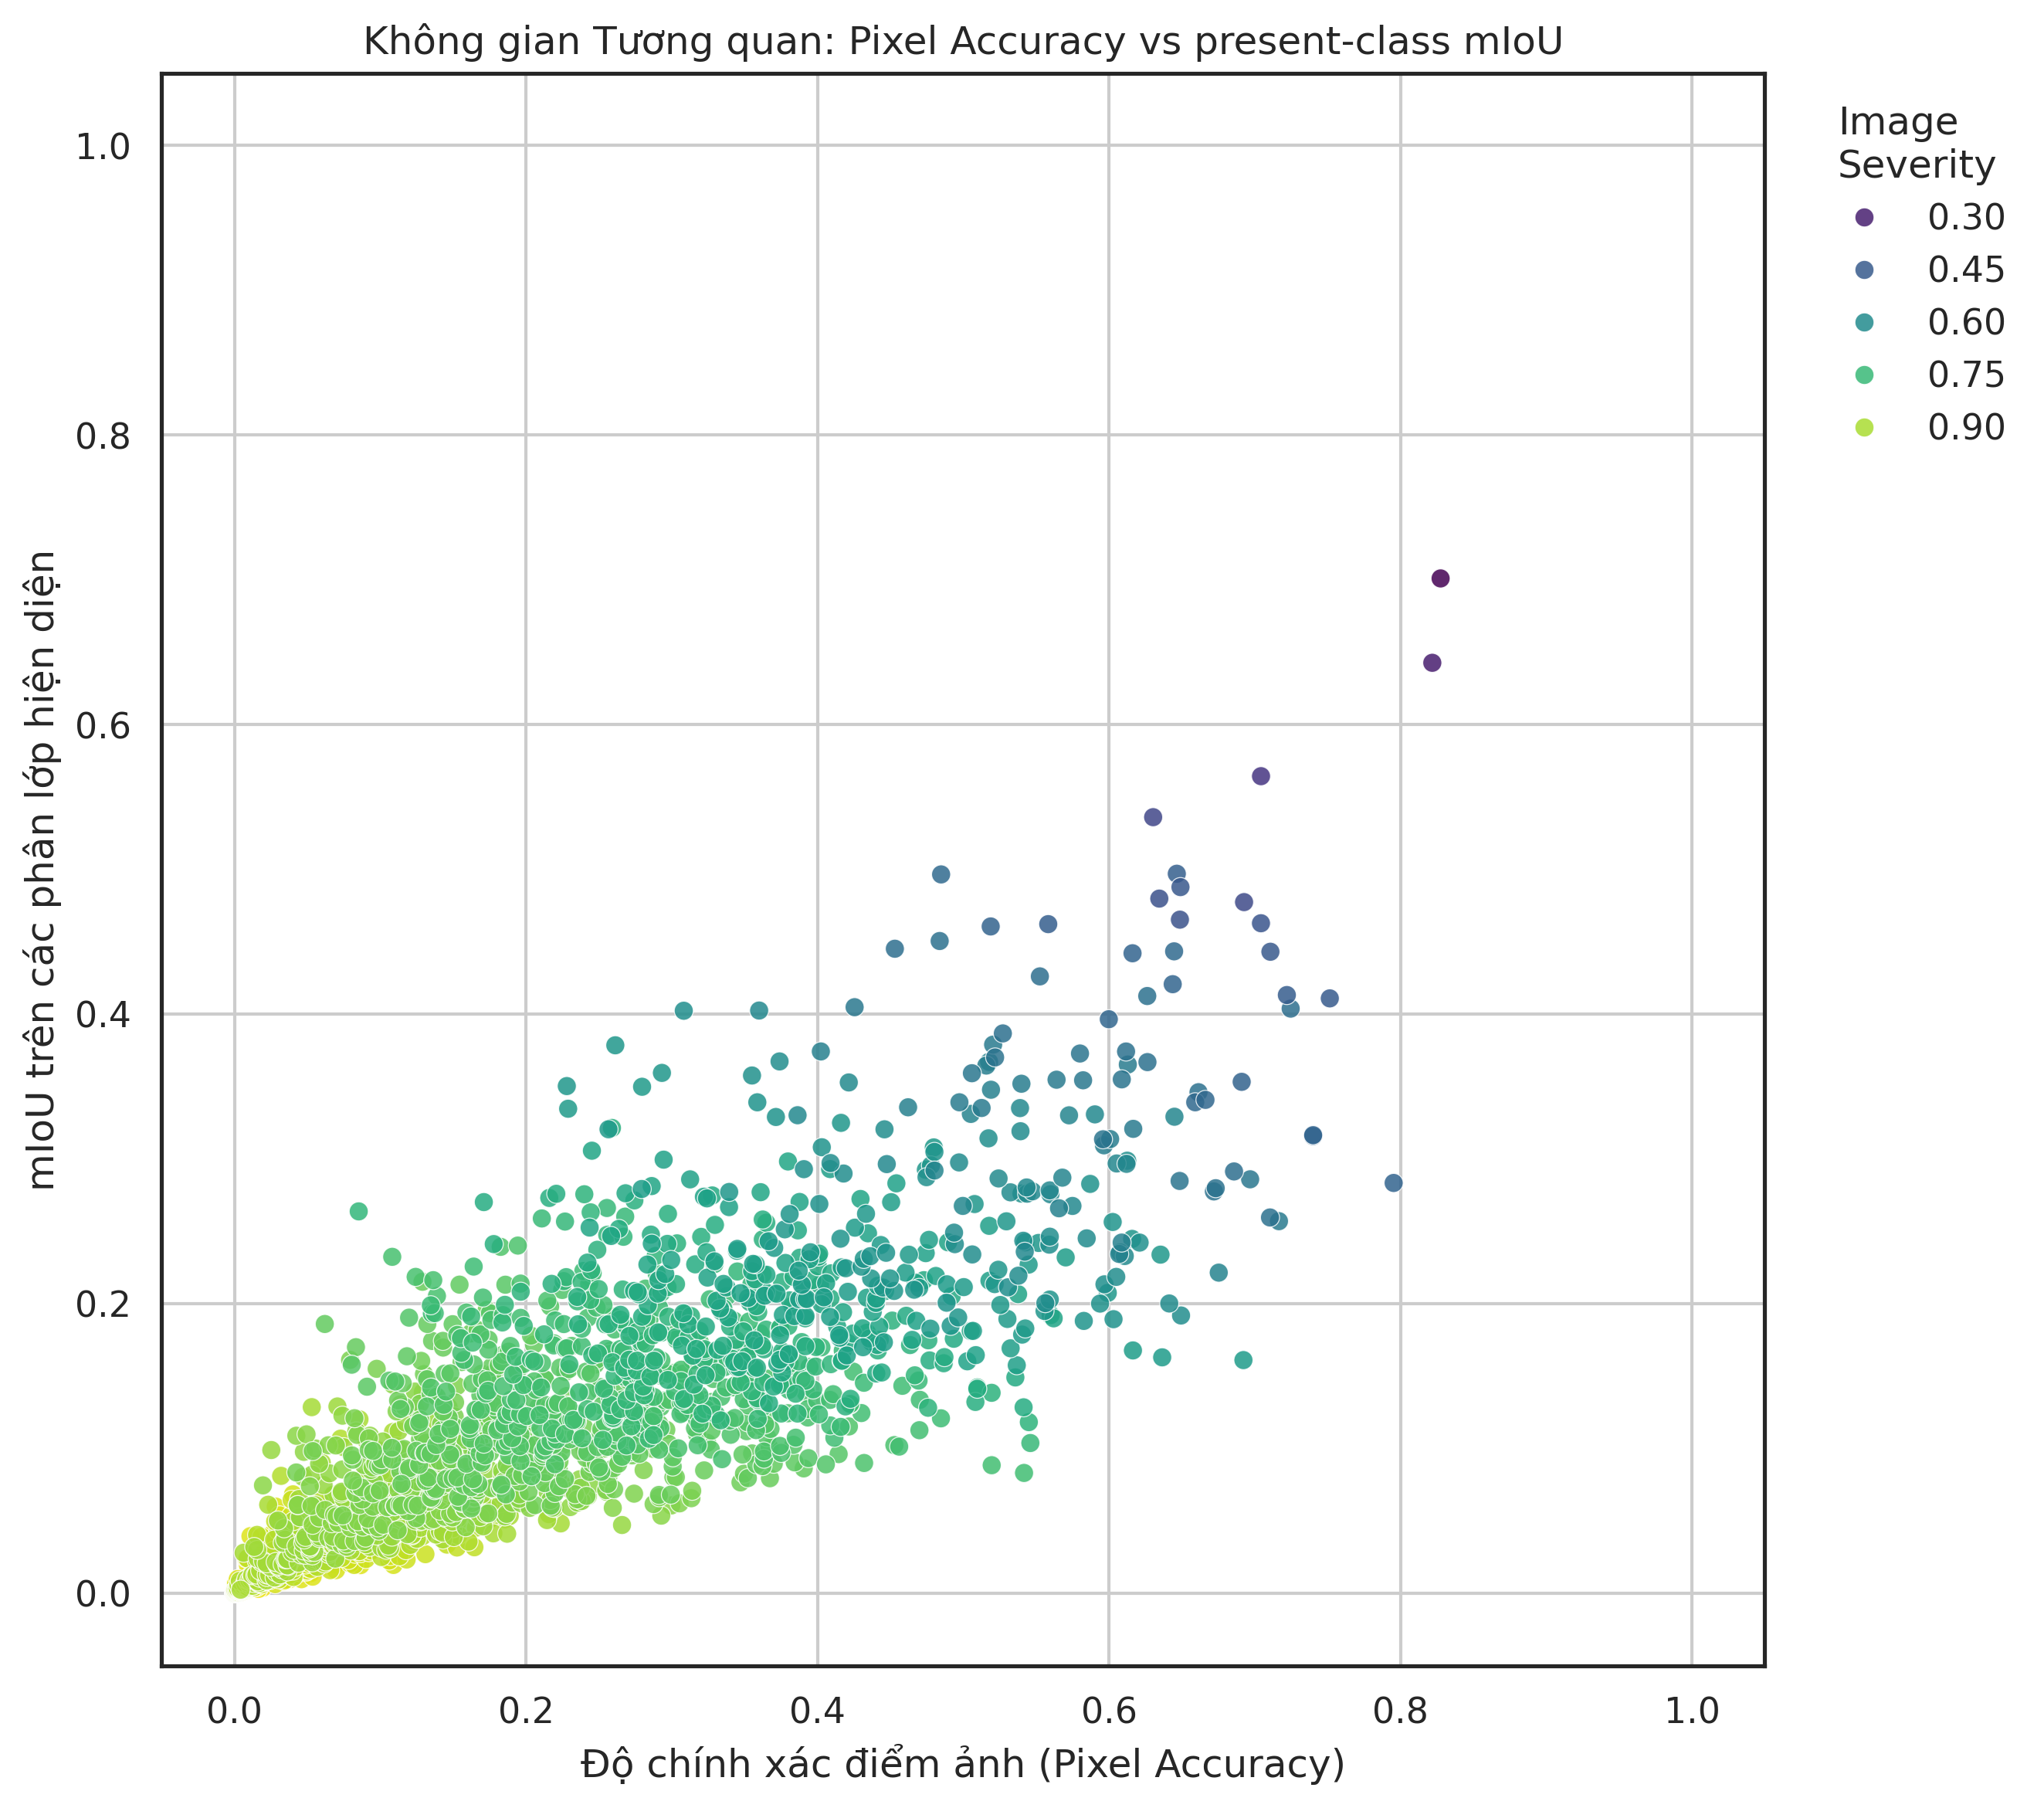
\includegraphics[width=\linewidth]{img/analyze/eval-model/03_pixel_acc_vs_present_miou_improved.png}
        \caption{Pixel accuracy và present-class mIoU.}
        \label{fig:pixel_acc_vs_miou}
    \end{subfigure}
    \hfill
    \begin{subfigure}{0.49\linewidth}
        \centering
        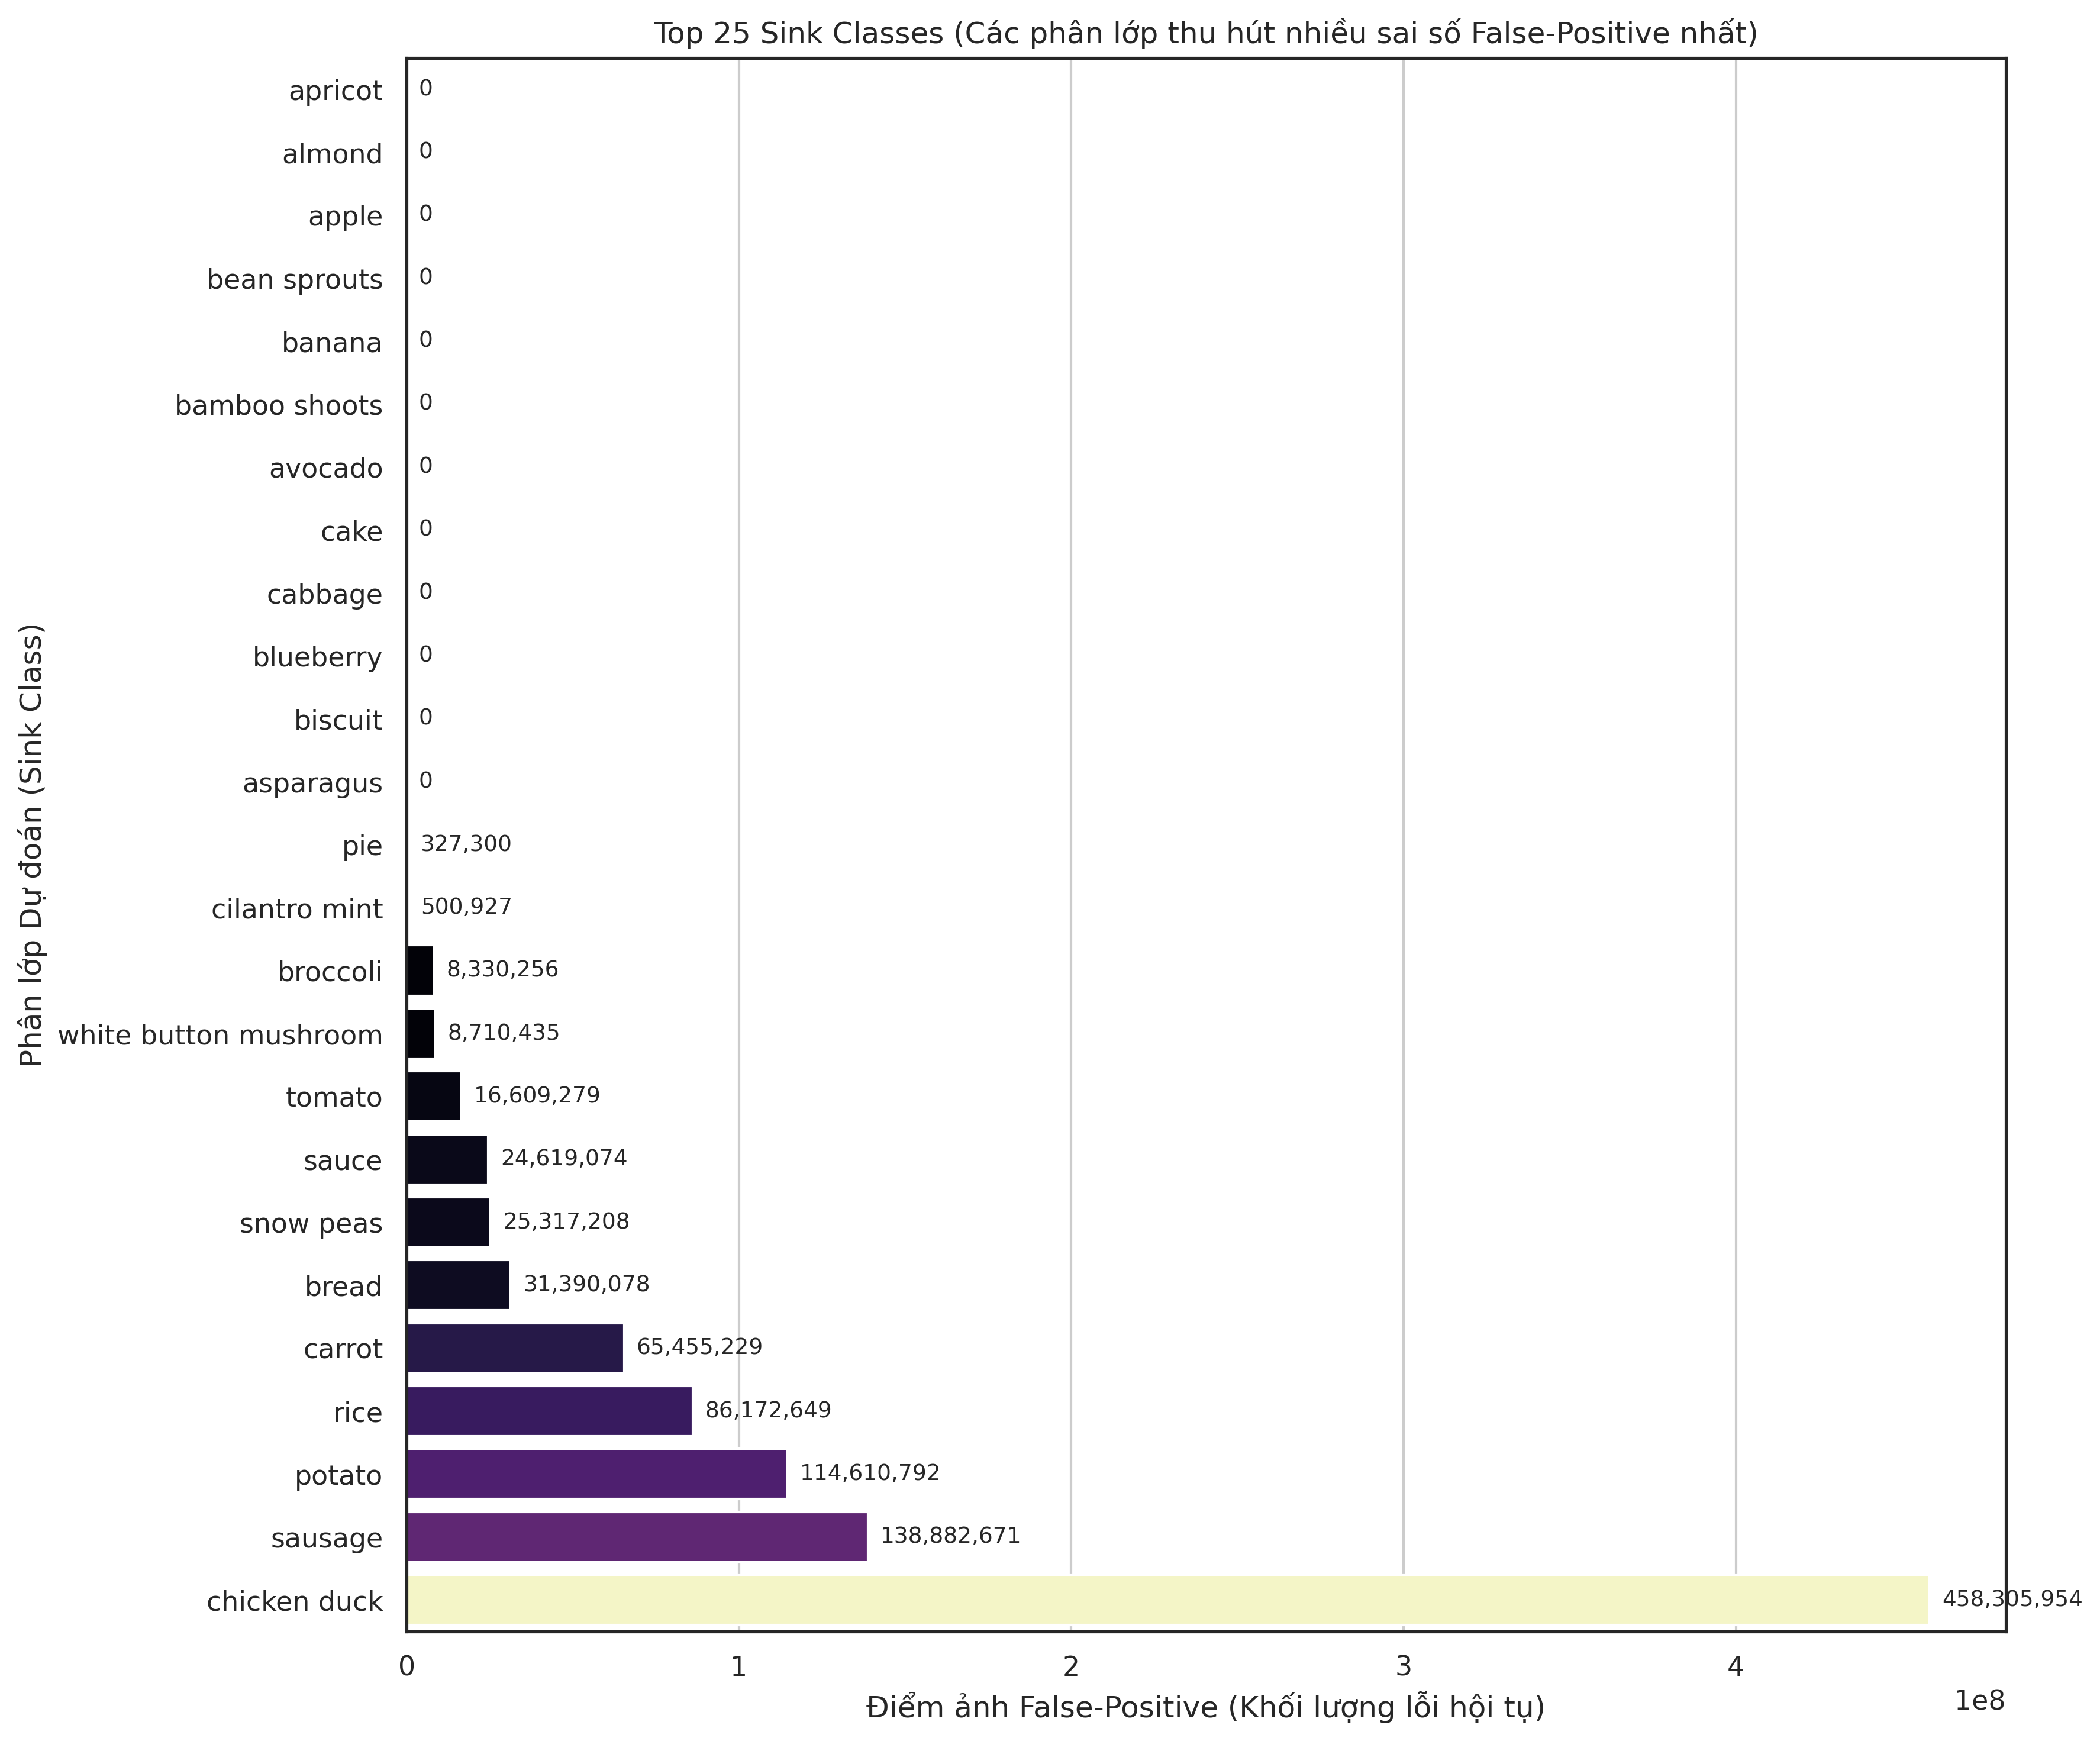
\includegraphics[width=\linewidth]{img/analyze/eval-model/05_top_sink_classes_improved.png}
        \caption{Top các sink classes thu hút false-positive.}
        \label{fig:sink_classes}
    \end{subfigure}
    \caption{Phân tích chất lượng mask và hiện tượng sink class của baseline BiSeNet.}
    \label{fig:baseline_quality_sink}
\end{figure}

Hình~\ref{fig:pixel_acc_vs_miou} cho thấy pixel accuracy và present-class mIoU có xu hướng đồng biến, nhưng không tương ứng tuyến tính. Nhiều mẫu có pixel accuracy ở mức tương đối khá, khoảng $0.3$--$0.6$, nhưng present-class mIoU vẫn thấp, phần lớn nằm dưới $0.3$. Điều này cho thấy baseline có thể dự đoán đúng nhiều pixel ở các vùng lớn hoặc vùng dễ, nhưng chất lượng mask theo từng lớp vẫn chưa tốt.

Nguyên nhân chính là pixel accuracy ít nhạy với lỗi trên lớp nhỏ và vùng biên, trong khi mIoU phạt đồng thời $FP$ và $FN$. Vì vậy, khi mask bị tràn sang vùng lân cận, bỏ sót nguyên liệu nhỏ hoặc nhầm sang lớp phổ biến, mIoU giảm mạnh dù pixel accuracy chưa giảm tương ứng. Kết quả này cho thấy điểm yếu của baseline không chỉ nằm ở nhận diện lớp, mà còn ở khả năng định vị chính xác vùng nguyên liệu.

\subsubsection{Phân tích lớp khó và sink class}

Hình~\ref{fig:sink_classes} cho thấy lỗi false-positive không phân bố đều giữa các lớp. Một số lớp đóng vai trò như ``sink class'', tức thu hút lượng lớn pixel từ các lớp khác. Nổi bật nhất là \textit{chicken duck} với khoảng $458.3$ triệu pixel false-positive, vượt xa các lớp tiếp theo như \textit{sausage} ($138.9$ triệu), \textit{potato} ($114.6$ triệu), \textit{rice} ($86.2$ triệu) và \textit{carrot} ($65.5$ triệu).

Hiện tượng này cho thấy baseline có xu hướng gom các vùng không chắc chắn vào một số lớp có biểu diễn thị giác rộng hoặc xuất hiện phổ biến. Các lớp như \textit{chicken duck}, \textit{sausage}, \textit{pork} và \textit{steak} đều có màu sắc sau chế biến khá gần nhau, bề mặt giàu texture và ranh giới không ổn định. Khi mô hình chưa học tốt đặc trưng texture cục bộ, các vùng thịt, bánh, sốt hoặc nền phức tạp dễ bị kéo về những lớp này.

Về mặt IoU, sink class gây lỗi kép: lớp nguồn tăng $FN$ vì pixel thật bị dự đoán sai, còn lớp sink tăng $FP$ vì nhận thêm pixel không thuộc về nó. Do đó, để cải thiện mIoU, chỉ tăng độ chính xác tổng thể là chưa đủ; cần giảm thiên lệch dự đoán về các lớp sink và tăng khả năng phân biệt texture giữa các lớp có hình thái gần nhau.

\subsubsection{Phân tích ma trận nhầm lẫn}

\begin{figure}[H]
    \centering
    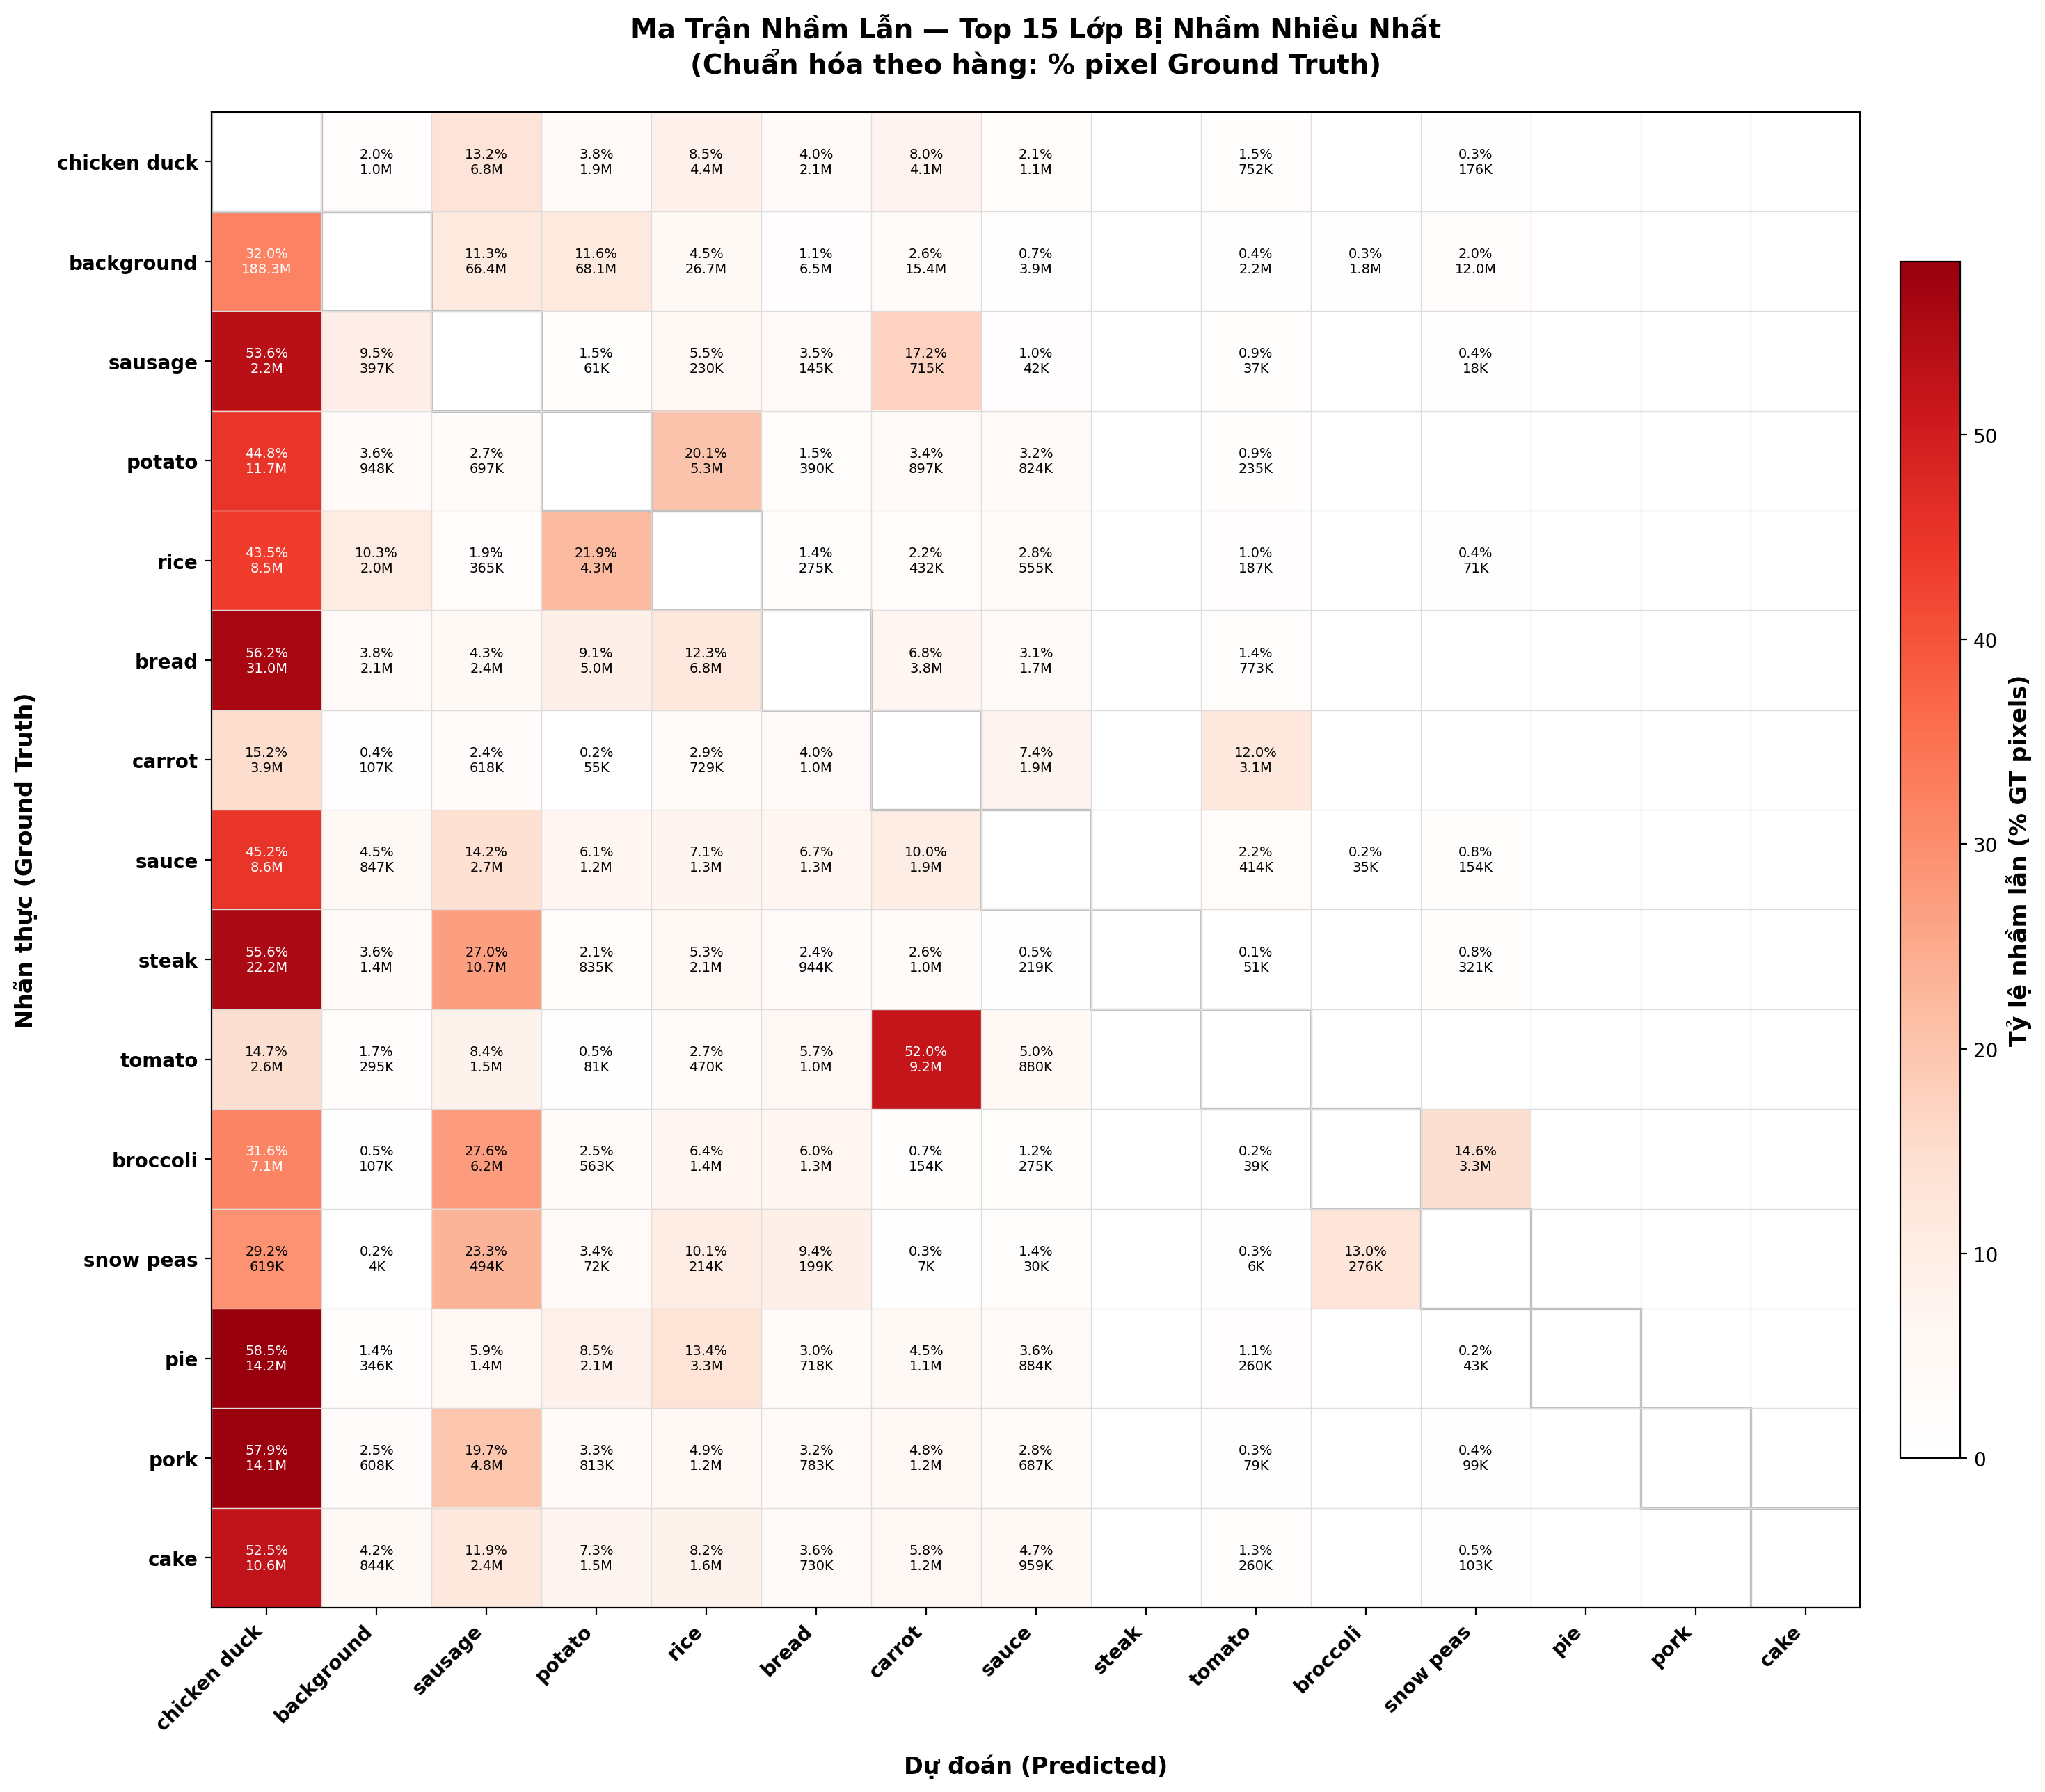
\includegraphics[width=\linewidth]{img/analyze/eval-model/04_top_confusion_directions_improved.png}
    \caption{Ma trận nhầm lẫn của các lớp bị nhầm nhiều nhất, chuẩn hóa theo hàng theo phần trăm pixel ground truth.}
    \label{fig:confusion_matrix}
\end{figure}

Hình~\ref{fig:confusion_matrix} cho thấy các lỗi nhầm lẫn của baseline có cấu trúc rõ ràng. Nhiều lớp bị dự đoán mạnh sang \textit{chicken duck}, ví dụ \textit{pie} ($58.5\%$), \textit{pork} ($57.9\%$), \textit{bread} ($56.2\%$), \textit{steak} ($55.6\%$), \textit{sausage} ($53.6\%$) và \textit{cake} ($52.5\%$). Ngay cả \textit{background} cũng có $32.0\%$ pixel bị dự đoán thành \textit{chicken duck}, tương ứng khoảng $188.3$ triệu pixel.

\begin{figure}[H]
    \centering
    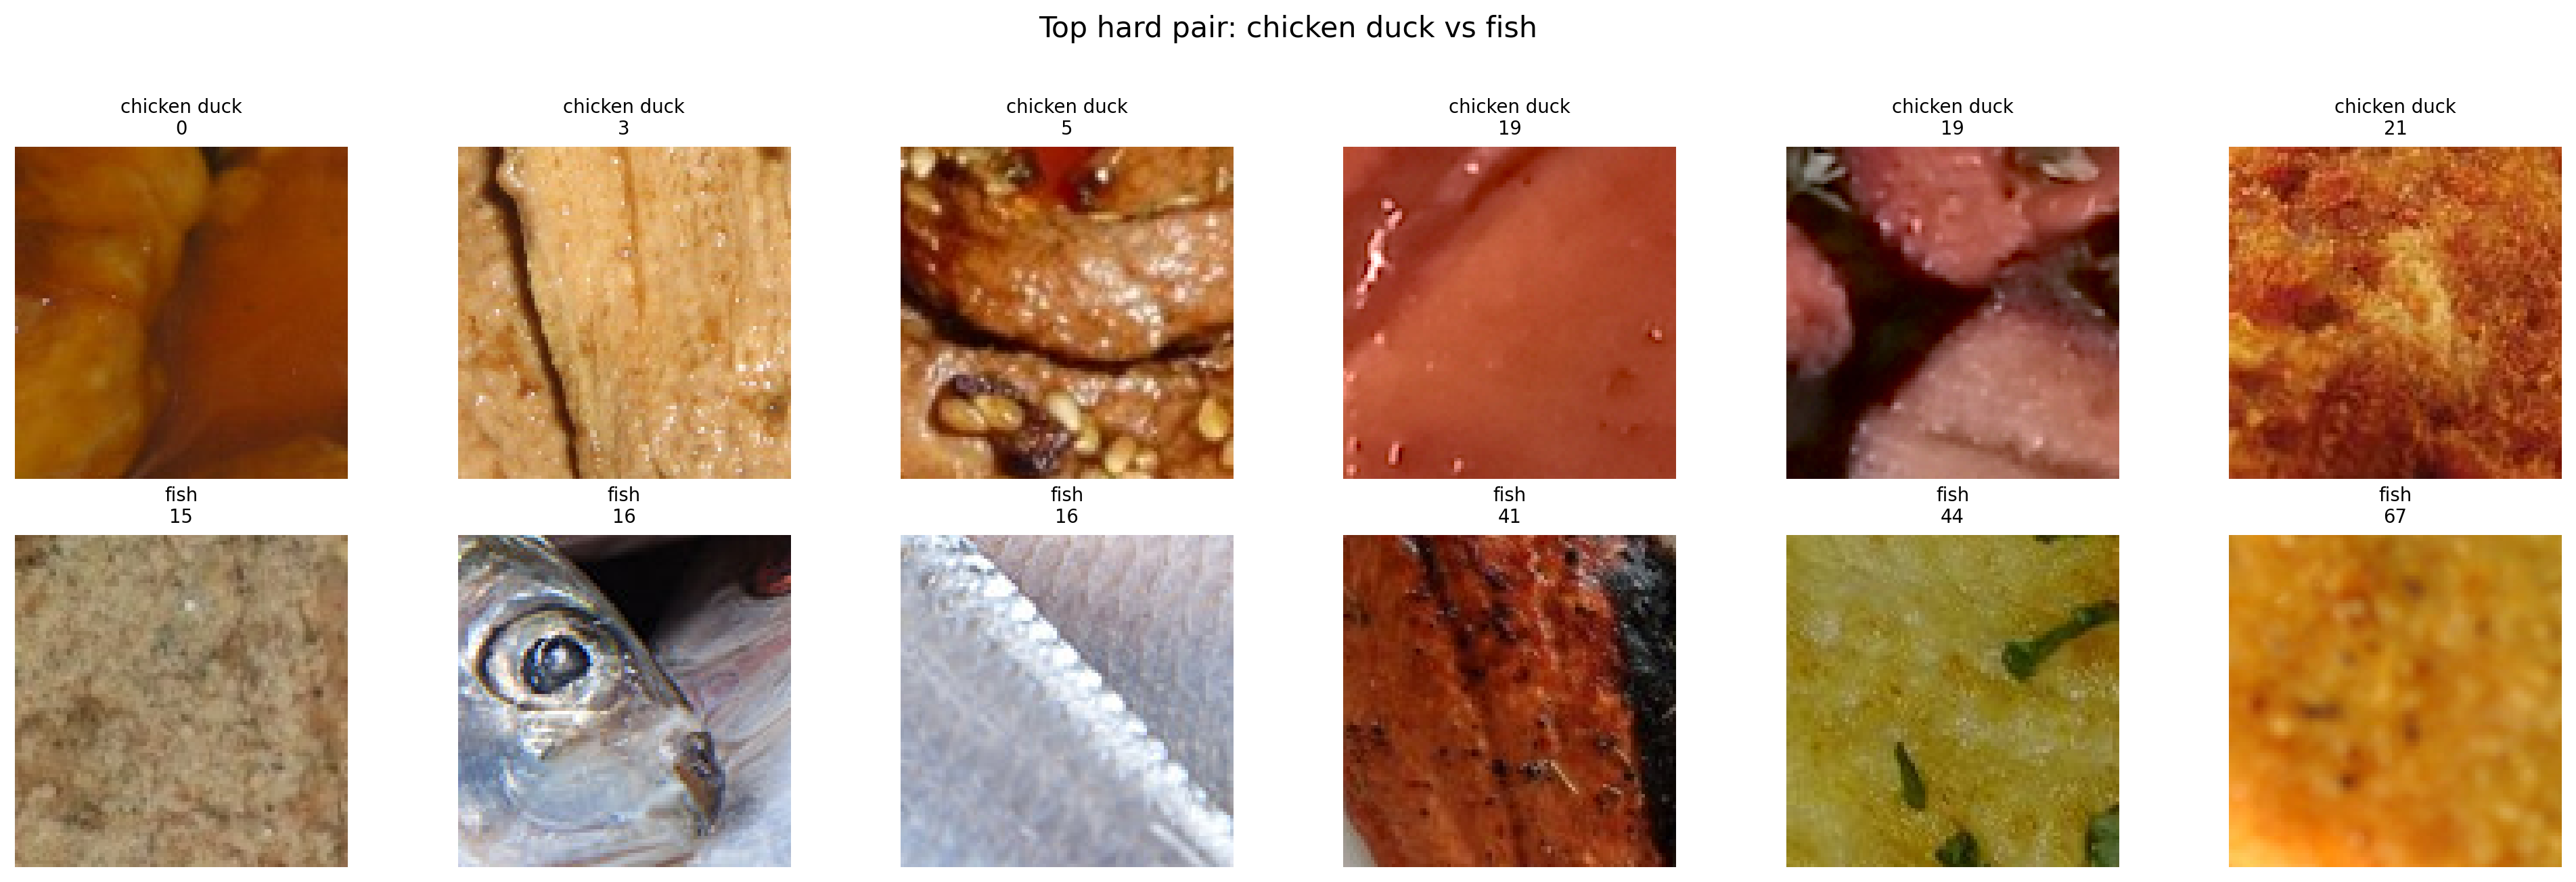
\includegraphics[width=\linewidth]{img/analyze/top_hard_pair_gallery.png}
    \caption{Top hard pair gallery: các patch mẫu của cặp nhầm lẫn khó \textit{chicken duck} và \textit{fish}.}
    \label{fig:top_hard_pair_gallery}
\end{figure}

Ngoài lỗi hút về một lớp trung tâm, ma trận còn cho thấy các cặp nhầm lẫn có ý nghĩa thị giác hoặc ngữ cảnh. Ví dụ, \textit{rice} bị nhầm sang \textit{potato} ($21.9\%$), và \textit{potato} bị nhầm sang \textit{rice} ($20.1\%$). Các lớp có bề mặt hoặc màu sắc gần nhau cũng bị nhầm đáng kể, như \textit{steak} $\rightarrow$ \textit{sausage} ($27.0\%$), \textit{broccoli} $\rightarrow$ \textit{sausage} ($27.6\%$), và \textit{sauce} $\rightarrow$ \textit{sausage} ($14.2\%$).

Các kết quả này cho thấy lỗi của baseline không phải là ngẫu nhiên. Mô hình đang bị ảnh hưởng bởi hai yếu tố: tương đồng texture giữa các nguyên liệu và quan hệ đồng xuất hiện trong ảnh món ăn. Spatial Path của BiSeNet giúp giữ một phần chi tiết không gian, nhưng chưa đủ để phân biệt texture fine-grained. Context Path học ngữ cảnh toàn cục, nhưng nếu thiếu cơ chế kiểm soát quan hệ lớp, nó có thể làm tăng thiên lệch về các lớp thường xuất hiện hoặc lớp có biểu diễn rộng.